\section{Diseño propuesto}

\subsection{Tipos de ondas}

Los tipos de ondas propuestos son los que se observan en la Figura \ref{fig:tipos-de-ondas} y Figura \ref{fig:senoidal}

\begin{figure}[H]
    \centering
    \includegraphics[width=0.5\linewidth]{tipos-de-onda.png}
    \label{fig:tipos-de-ondas}
\end{figure}    
\begin{figure}[H]
    \centering
    \includegraphics[width=0.5\linewidth]{senoidal.png}
    \label{fig:senoidal}
\end{figure}    

\subsection{Diagrama en bloques del circuito}
\resizebox{\textwidth}{!}{
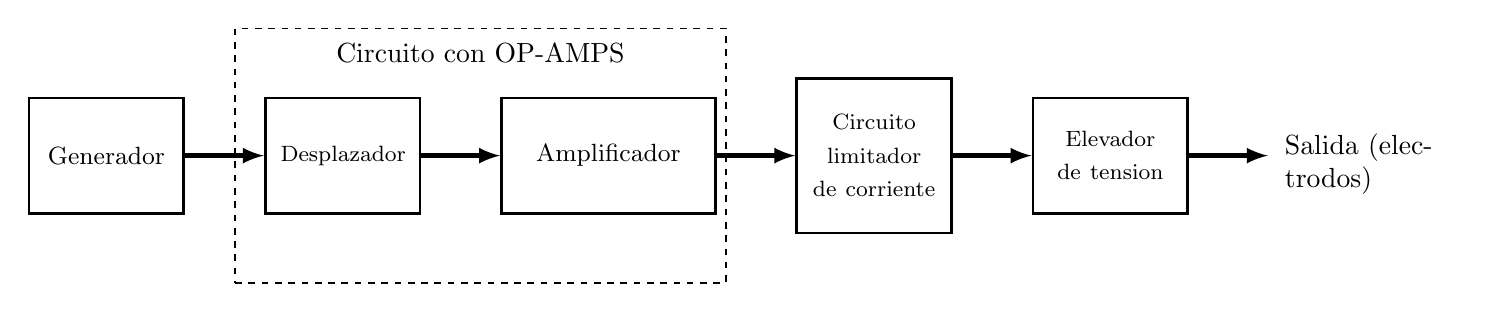
\begin{tikzpicture}
	% Paths, nodes and wires:
	\node[shape=rectangle, draw, line width=1pt, minimum width=1.965cm, minimum height=1.465cm] at (5, 6.5){} node[anchor=center, align=center, text width=1.711cm, inner sep=4.1pt] at (5, 6.5){\small Generador};
	\draw[line width=1.6pt, -latex] (6, 6.5) -- (7, 6.5);
	\node[shape=rectangle, draw, line width=1pt, minimum width=1.965cm, minimum height=1.465cm] at (8, 6.5){} node[anchor=center, align=center, text width=1.577cm, inner sep=6pt] at (8, 6.5){\footnotesize Desplazador};
	\draw[line width=1.6pt, -latex] (9, 6.5) -- (10, 6.5);
	\node[shape=rectangle, draw, line width=1pt, minimum width=2.715cm, minimum height=1.465cm] at (11.375, 6.5){} node[anchor=center, align=center, text width=2.327cm, inner sep=6pt] at (11.375, 6.5){\small Amplificador};
	\node[shape=rectangle, draw, line width=0.6pt, dash pattern={on 2.4pt off 2.4pt}, minimum width=6.229cm, minimum height=3.229cm] at (9.75, 6.5){} node[anchor=north, align=center, text width=5.855cm, inner sep=5.6pt] at (9.75, 8.125){Circuito con OP-AMPS};
	\draw[line width=1.6pt, -latex] (12.75, 6.5) -- (13.75, 6.5);
	\node[shape=rectangle, draw, line width=1pt, minimum width=1.965cm, minimum height=1.465cm] at (17.75, 6.5){} node[anchor=center, align=center, text width=1.711cm, inner sep=4.1pt] at (17.75, 6.5){\footnotesize Elevador de tension};
	\draw[line width=1.6pt, -latex] (15.75, 6.5) -- (16.75, 6.5);
	\node[shape=rectangle, draw, line width=1pt, minimum width=1.965cm, minimum height=1.965cm] at (14.75, 6.5){} node[anchor=center, align=center, text width=1.711cm, inner sep=4.1pt] at (14.75, 6.5){\footnotesize Circuito\\limitador de corriente};
	\draw[line width=1.6pt, -latex] (18.75, 6.5) -- (19.75, 6.5);
	\node[shape=rectangle, minimum width=2.465cm, minimum height=1.215cm] at (21, 6.375){} node[anchor=north west, align=left, text width=2.077cm, inner sep=6pt] at (19.75, 7){Salida (electrodos)};
\end{tikzpicture}}
